%!TEX root = thesis.tex
%-------------------------------------------------------------------------------
\chapter{Bounding the standard quantum value of extended nonlocal games}
\label{chap:extended_npa_hierarchy}
%-------------------------------------------------------------------------------

In this chapter, we shall present a number of heuristic methods that obtain bounds on the standard quantum value of an extended nonlocal game. For placing upper bounds, we take inspiration from the QC hierarchy~\cite{Doherty2008, Navascues2007,Navascues2008}; a hierarchy of semidefinite programs that yield progressively better upper bounds on the quantum value for nonlocal games as one computes higher levels of the hierarchy. Indeed, we adopt these results and provide what we refer to as the \index{extended QC hierarchy}{\emph{extended QC hierarchy}} and apply this technique to the class of extended nonlocal games to obtain upper bounds on the standard quantum value. 

In Section~\ref{sec:extended-npa-hierarchy}, we present the extended QC hierarchy in greater detail. We begin in Section~\ref{sec:intuitive-description-of-the-extended-qc-hierarchy} by giving an informal description of how the extended QC hierarchy is structured. In Section~\ref{sec:construction-of-the-extended-qc-hierarchy}, we make this description more formal and show in Section~\ref{sec:convergence-of-the-extended-qc-hierarchy} that the extended QC hierarchy has a similar convergence property as does the original QC hierarchy. In Section~\ref{sec:examples-upper-bounds-extended-npa}, we shall provide some explicit examples of how one may apply the extended QC hierarchy to extended nonlocal games. 

In Section~\ref{sec:lower-bound-extended-nonlocal-games}, we present our method to lower bound the value of extended nonlocal games which is inspired by the work of Liang and Doherty~\cite{Liang2007}, where they consider a method that can be applied to lower bound the quantum value in the nonlocal game setting. We adopt their technique and apply it to the case of extended nonlocal games. In Section~\ref{sec:examples-lower-bounds}, we provide explicit examples of applying this lower bound technique to an extended nonlocal game. 

This chapter is based on joint work with Nathaniel Johnston, Rajat Mittal, and John Watrous~\cite{Johnston2015a}.  

\minitoc

%-------------------------------------------------------------------------------
\section{Upper bounds for extended nonlocal games: the extended QC hierarchy}
\label{sec:extended-npa-hierarchy}
%-------------------------------------------------------------------------------

In this section we describe how the original \index{QC hierarchy}{\emph{QC hierarchy}}~\cite{Doherty2008,Navascues2007, Navascues2008}, may be generalized to extended nonlocal games. The QC hierarchy is a method that allows one to obtain upper bounds on the quantum value of a nonlocal game. Specifically, for a finite level, the commuting measurement value of a nonlocal game is guaranteed to be obtained, which serves as a natural upper bound to the quantum value of a nonlocal game. Directly calculating the quantum value of a nonlocal game is probably intractable, but in most cases, the first few levels of the QC hierarchy are numerically tractable to compute on current hardware, and in many cases the first few levels are sufficient~\cite{Pal2009}. 

%-------------------------------------------------------------------------------
\subsection{Intuitive description of the extended QC hierarchy} \label{sec:intuitive-description-of-the-extended-qc-hierarchy}
%-------------------------------------------------------------------------------

In this section, we shall provide some intuition on how one may interpret and use the extended QC hierarchy. Many of these ideas are also found in the QC hierarchy for nonlocal games. First, let us establish what the extended QC hierarchy is used for: it is a technique to allow one to place upper bounds on the standard quantum value of a given extended nonlocal game. More precisely, it is a method that allows us to obtain the commuting measurement value of a given extended nonlocal game, where it may be recalled from Chapter~\ref{chap:extended_nonlocal_games}, that the commuting measurement value is an upper bound on the standard quantum value for every extended nonlocal game, that is $\omega^*(G) \leq \omega_c(G)$ holds for any extended nonlocal game $G$. 

Recall that the commuting measurement value of an extended nonlocal game is given by a maximization over the following equation
\begin{align} \label{eq:commuting-meas-val-eqchier}
	\sum_{(x,y) \in \Sigma} \pi(x,y) \sum_{(a,b) \in \Gamma} \biggip{V(a,b|x,y)}{K(a,b|x,y)},
\end{align}
where $K$ is a commuting measurement assemblage operator. What the extended QC hierarchy allows us to do is to consider the following equation instead to compute the commuting measurement value
\begin{align} \label{eq:eqchier-val}
	\sum_{(x,y) \in \Sigma} \pi(x,y) \sum_{(a,b) \in \Gamma} \biggip{V(a,b|x,y)}{M^{(k)}(a,b|x,y)},
\end{align}
where now $M^{(k)}$ is some matrix parametrized by some integer $k$ with entries indexed by $a \in \GammaA$, $b \in \GammaB$, $x \in \SigmaA$, and $y \in \SigmaB$ satisfying certain constraints, which we will elaborate on shortly. The benefit of this is that we can optimize over the matrix $M^{(k)}$ and these constraints for some level $k$ by way of a semidefinite program, and thereby compute the commuting measurement value of an extended nonlocal game. Of course, showing that such a correspondence exists between equations~\eqref{eq:commuting-meas-val-eqchier} and~\eqref{eq:eqchier-val} is the difficult part, and is what we will be showing in Theorem~\ref{thm:extended-npa-convergence} in Section~\ref{sec:convergence-of-the-extended-qc-hierarchy}. 

Assuming that there does exist such a correspondence though, let us consider what the $M^{(k)}$ matrices look like, and how to compute the constraints on these matrices as the level $k$ increases. These matrices can be thought to embody certain properties that one would expect from a commuting measurement strategy. That is to say that the entries in the matrices $M^{(k)}$ are indexed by strings which correspond to operators coming from a commuting measurement strategy. It may be recalled that the measurements for such a strategy obey pair-wise commutative properties, sum to the identity when summing over the outputs, and may be considered to be projective without any loss of generality. The strings within these matrices possess these qualities in ways that we will describe. 

Assume that question and answer alphabets $\SigmaA$, $\SigmaB$, $\GammaA$, and
$\GammaB$, as well as a positive integer $m$ representing the dimension of the
referee's quantum system, have been fixed. The symbol $\cupdot$ denotes the disjoint union, meaning that $\SigmaA \times \GammaA$ and
$\SigmaB \times \GammaB$ are to be treated as disjoint sets when forming
\begin{align}
\Delta = \left( \SigmaA \times \GammaA \right) \cupdot \left( \SigmaB \times \GammaB \right).
\end{align}
We write $\Delta^{\ast}$ to denote the set of all strings (of finite length) over
$\Delta$, and we write $\varepsilon$ to denote the empty string.

For simplicity, we will restrict our attention to $k = 1$, the first level of the extended QC hierarchy, and consider an extended nonlocal game where the dimension of the referee's space is $r$ and the game consists of $n$ possible questions and $m$ possible answers for each player. The matrix $M^{(1)}$ consists $r \times r$ blocks
\begin{align}
	M^{(1)} = \begin{pmatrix}
				M_{1,1}^{(1)} & \cdots & M^{(1)}_{1,r} \\
				\vdots & \ddots & \vdots \\
				M_{m,1}^{(1)} & \cdots & M_{r,r}^{(1)}
			   \end{pmatrix}.
\end{align}
We construct each block $M_{i,j}^{(1)}$ by lining all tuples of strings that correspond to measurement operators and the identity operator used in the extended nonlocal game. For instance, the tuple $(x,a)$ can be thought of a string pair that corresponds to Alice's measurement operator $A_a^x$. We use $\epsilon$ as the empty string that relates to the identity operator. More specifically, for $k = 1$, we consider all strings of length at most one from the set
\begin{align}
	\Delta^{\leq 1} = \{\varepsilon\} \cup \left \{ (x,a) \right \} \cup \left \{ (y,b) \right \}.
\end{align}
The block matrices are then formed from this set as $M_{i,j}^{(1)} : \Delta^{\leq 1} \times \Delta^{\leq 1}$ where $1 \leq i,j \leq r$.  This is a bit clearer if we simply write out what we have described thus far 
\begin{footnotesize}
\[
\begin{aligned}
M_{i,j}^{(1)} =
\left(
\begin{array}{c||cccc|ccc}
 & \epsilon & (x_1,a_1) & \cdots & (x_{nm},a_{nm}) & (y_1,b_1) & \cdots & (y_{nm},b_{nm}) \\
\hline\hline 
\epsilon & & & & & & & \\
(x_1,a_1) & & & & & & & \\
\vdots & & & & & & & \\
(x_{nm},a_{nm}) & & & & & & & \\
\hline 
(y_1,b_1) & & & & & & & \\
\vdots & & & & & & & \\
(y_{nm},b_{nm}) & & & & & & &
\end{array}
\right). 
\end{aligned}
\]
\end{footnotesize}
Now we have not actually placed an entry into this matrix yet. The outer row and outer column are simply guides we will use to fill in the matrix. Specifically, we fill the matrix by composing the outer row element with the outer column element. Again, writing this out explicitly may enhance the explanation,
\begin{tiny}
\[
\begin{aligned}
M_{i,j}^{(1)} =
\left(
\begin{array}{c||cccc|ccc}
 & \epsilon & (x_1,a_1) & \cdots & (x_{nm},a_{nm}) & (y_1,b_1) & \cdots & (y_{nm},b_{nm}) \\
\hline\hline 
\epsilon & \epsilon & (x_1,a_1) & \cdots & (x_{nm},a_{nm}) & (y_1,b_1) & \cdots & (y_{nm},b_{nm}) \\
(x_1,a_1) & (x_1,a_1) & (x_1,a_1) & \cdots & (x_1,a_1) (x_{nm},a_{nm}) & (x_1,a_1) (y_1,b_1) & \cdots & (x_1,a_1) (y_{nm},b_{nm}) \\
\vdots & \vdots & \vdots & \ddots & \vdots & \vdots  & \ddots & \vdots \\
(x_{nm},a_{nm}) & (x_{nm},a_{nm}) & (x_{nm},a_{nm}) (x_1,a_1) & \cdots & (x_{nm},a_{nm}) & (x_{nm},a_{nm}) (y_1,b_1) & \cdots & (x_{nm},a_{nm}) (y_{nm},b_{nm}) \\
\hline 
(y_1,b_1) & (y_1,b_1) & (y_1,b_1) (x_1,a_1) & \cdots & (y_1,b_1) (x_{nm},a_{nm}) & (y_1,b_1) & \cdots & (y_1,b_1) (y_{nm},b_{nm}) \\
\vdots & \vdots & \vdots & \ddots & \vdots & \vdots  & \ddots & \vdots \\
(y_{nm},b_{nm}) & (y_{nm},b_{nm}) & (y_{nm},b_{nm}) (x_1,a_1) & \cdots & (y_{nm},b_{nm}) (x_{nm},a_{nm}) & (y_{nm},b_{nm}) (y_1,b_1) & \cdots & (y_{nm},b_{nm})
\end{array}
\right). 
\end{aligned}
\]
\end{tiny}
Consider the last entry in the second row with entry $(x_1,a_1)(y_{nm},b_{nm})$. To obtain this entry, we multiplied, or more precisely, concatenated string pairs $(x_1,a_1)$, coming from the outer column, with the pair $(y_{nm},b_{nm})$, coming from the outer row. 

It is also essential to consider the first row, first column, and diagonal of $M_{i,j}^{(1)}$. Note how there is just a single element in these spots instead of two concatenated tuples. The reasoning behind this is that, as mentioned before, the properties of this matrix are meant to embody those of commuting measurement strategy. Take for instance the first entry in $M_{i,j}^{(1)}$ which is equal to just $\epsilon$. We would expect an entry of $\epsilon \epsilon$, but recall $\epsilon$ corresponds to the identity operator and $\I \I = \I$. In a similar way, the second entry in the second row is just $(x_1,a_1)$. Again, we would expect an entry of $(x_1,a_1)(x_1,a_1)$, however since we may assume that strings representing the measurements are projective, that is $A_{a_1}^{x_1} A_{a_1}^{x_1} = A_{a_1}^{x_1}$, this property is conveyed in a similar way. The same idea applies to the entire diagonal of $M_{i,j}^{(1)}$. 

We now consider how the commutation relationships are conveyed in this matrix. In $M_{i,j}^{(1)}$, this property is represented as enforcing that 
\begin{align}
	M^{(1)}_{i,j}((x,a),(y,b)) = M^{(1)}_{i,j}((y,b),(x,a)),
\end{align}
for all $(i,j)$ blocks. For instance, consider the entries $(y_1,b_1)(x_1,a_1)$ and $(x_1,a_1)(y_1,b_1)$. These entries are equal since the strings represent operators coming from a commuting measurement strategy, that is to say they represent the property 
\begin{align}
	\left[A_{a_1}^{x_1}, B_{b_1}^{y_1} \right] = \left[ B_{b_1}^{y_1}, A_{a_1}^{x_1} \right] = 0.
\end{align}
We also need to convey the property that the measurements of Alice and Bob are equal to the identity when summing over all answers. This is conveyed by observing that
\begin{equation}
	\begin{aligned}
		\sum_{a \in \GammaA} M^{(1)}((x,a),(y,b)) &= M^{(1)}(\epsilon,(y,b)), \\
		\sum_{b \in \GammaB} M^{(1)}((x,a),(y,b)) &= M^{(1)}((x,a),\epsilon).
	\end{aligned}
\end{equation}
The last constraint we place on the matrix $M^{(1)}$ is that it must be positive semidefinite. If this constraint, along with all of the other constraints regarding the blocks of $M^{(1)}$ are enforced, we refer to $M^{(1)}$ as a first-order admissible matrix, which will be formally defined in the coming sections for any $k$. Optimizing over such a matrix subject to the above conditions while attempting to maximize equation~\eqref{eq:eqchier-val} will provide us with our desired upper bound on the standard quantum value for some extended nonlocal game. 

It may happen that the first level of the hierarchy is not sufficient in attaining the true commuting measurement value. Specifically, the value at the first level may be higher than the actual commuting measurement value. In this case, computing higher levels of $k$ will help us in getting closer to the true commuting measurement value. When constructing the block matrices $M^{(k)}_{i,j}$ for some level $k$, each block will have the following form
\begin{align}
	M_{i,j}^{(k)} : \Delta^{\leq k} \times \Delta^{\leq k} \rightarrow \complex,
\end{align} 
where 
%\begin{equation}
%	\begin{aligned}
%		\Delta^{\leq 0} &= \{ \varepsilon \}, \\
%		\Delta^{\leq 1} &= \Delta^{\leq 0} \cup \left \{ (x,a) : x \in \SigmaA^{\leq 1}, \ a \in \GammaA^{\leq 1} \right \} \cup \left \{ (y,b) : y \in \SigmaB^{\leq 1}, \ b \in \GammaB^{\leq 1}  \right \}, \\
%		\Delta^{\leq 2} &= \Delta^{\leq 1} \cup \{ (x,a), (x^{\prime},a^{\prime} : x,x^{\prime} \in \SigmaA^{\leq 2}, \ a,a^{\prime} \in \GammaA^{\leq 2} \} \\ 
%		& \qquad \quad \ \cup \{ (x,a), (y,b) : x \in \SigmaA^{\leq 2}, \ y \in \SigmaB^{\leq 2}, \ a \in \GammaA^{\leq 2}, \ b \in \GammaB^{\leq 2} \} \\ 			& \qquad \quad \ \cup \{ (y,b), (y^{\prime},b^{\prime}) : y, y^{\prime} \in \SigmaB^{\leq 2}, \ b,b^{\prime} \in \GammaB^{\leq 2} \}, \\
%		\vdots
%	\end{aligned}
%\end{equation}
\begin{equation}
	\begin{aligned}
		\Delta^{\leq 0} &= \{ \varepsilon \}, \\
		\Delta^{\leq 1} &= \Delta^{\leq 0} \cup \{ (x,a) \} \cup \{ (y,b) \}, \\
		\Delta^{\leq 2} &= \Delta^{\leq 1} \cup \{ (x,a)(x^{\prime},a^{\prime}) \} \cup \{ (x,a)(y,b) \} \cup \{ (y,b)(y^{\prime},b^{\prime}) \}, \\
		\vdots
	\end{aligned}
\end{equation}
where $x \not= x^{\prime}$, $a \not= a^{\prime}$, $y \not= y^{\prime}$, and $b \not= b^{\prime}$. It is apparent that as $k$ increases, the alphabets have the following property that 
\begin{align}
	\Delta^{\leq 0} \subseteq \Delta^{\leq 1} \subseteq \cdots \subseteq \Delta^{\leq k}.
\end{align}
That is to say, the blocks in $M^{(k)}$ will consist of more and more entries as $k$ increases. One of the main ideas of the extended QC hierarchy that is also similar to the original QC hierarchy is that as $k$ increases, this leads to better and better approximations of the commuting measurement value of some extended nonlocal game $G$, that is
\begin{align}
	\omega_c^k(G) \leq \cdots \leq \omega_c^{2}(G) \leq \omega_c^1(G),
\end{align}
for some value of $k$. This relationship is depicted in Figure~\ref{fig:qc-hierarchy-levels}. 

\begin{figure}[!htpb] 
	\begin{center}
		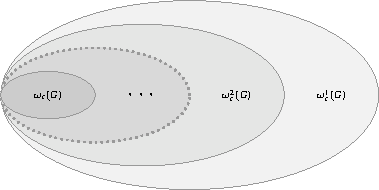
\includegraphics[scale=1.5]{figures/qc_hierarchy_levels.pdf}
	\end{center}
		\caption[Levels of the extended QC hierarchy.]{A visual representation of computing levels of the extended QC hierarchy. The outermost ellipse corresponds to the value attained when one computes the first level of the extended QC hierarchy. We represent this as $\omega^1_c(G)$, where $k=1$ represents the level computed. For certain games, this may indeed by equal to the true commuting measurement value of the game, that is $\omega_c(G)$.}
\label{fig:qc-hierarchy-levels}		
\end{figure}  

As previously mentioned, one nice property of the extended QC hierarchy that is also enjoyed by the QC hierarchy for nonlocal games is that obtaining the commuting measurement value is guaranteed for any extended nonlocal game for some finite level $k$. The downside to this, of course, is that $k$ may be particularly large. From an algorithm analysis perspective, the original QC hierarchy scales exponentially with respect to the level computed, that is $(nm)^k$, where again $n$ represents the total number of questions and $m$ represents the total number of answers. Indeed, for the extended QC hierarchy, the complexity fares even worse as we also have the referee's space to be concerned about now. It is therefore sometimes helpful to consider intermediate levels that are between integer values of $k$. For instance
\begin{equation}
	\begin{aligned}
		\Delta^{\leq 0} &= \{ \varepsilon \}, \\
		\Delta^{\leq 1} &= \Delta^{\leq 0} \cup \{ (x,a) \} \cup \{ (y,b) \}, \\
		\Delta^{\leq 1+AB} &= \Delta^{\leq 1} \cup \{ (x,a)(y,b) \}, \\
		\vdots
	\end{aligned}
\end{equation}
where $x \not= x^{\prime}$, $a \not= a^{\prime}$, $b \not= b^{\prime}$, and $y \not= y^{\prime}$. The $k = 1 + AB$ level is not quite as restrictive computationally as the complete second level of the hierarchy, and this may be enough in certain cases to obtain the commuting measurement value for a given extended nonlocal game. These intermediate levels have also been considered for the original QC hierarchy as well and serve a similar purpose. 

In practice, for many nonlocal games and extended nonlocal games, the values emerging from low levels of the QC hierarchy and extended QC hierarchy agree with the true commuting measurement value of the game. While there do exist some exceptions to this property, such as the I3322 game (based on the I3322 inequality~\cite{Collins2004}), the authors here~\cite{Pal2009} for instance were able to show a wide variety of Bell inequalities (or nonlocal games) that the QC hierarchy was able to obtain the commuting measurement value at low levels of the hierarchy.
 
In the next section, we will make our intuition developed in this section more formal, and we will further prove that the extended QC hierarchy allows one to obtain the commuting measurement value of any extended nonlocal game. Our proof technique for this follows very closely the technique used in~\cite{Navascues2007, Navascues2008} to prove convergence for the QC hierarchy for nonlocal games.


%-------------------------------------------------------------------------------
\subsection{Construction of the extended QC hierarchy} \label{sec:construction-of-the-extended-qc-hierarchy}
%-------------------------------------------------------------------------------

Define $\sim$ to be the equivalence relation on $\Delta^{\ast}$
generated by the following rules:\vspace{2mm}

\noindent
\begin{tabular}{@{\hspace*{1.2mm}}lll}
  1. \hspace*{-3mm} & $s \sigma t \sim s \sigma \sigma t$ & (for every
  $s,t\in\Delta^{\ast}$ and $\sigma \in \Delta$).\\[1mm]
  2. \hspace*{-3mm} & $s \sigma \tau t \sim s \tau \sigma t$ & 
  (for every $s,t\in\Delta^{\ast}$, $\sigma \in \SigmaA \times \GammaA$, and 
  $\tau\in \SigmaB \times \GammaB$).\\[2mm]
\end{tabular}

\noindent
That is, two strings are equivalent with respect to the relation $\sim$
if and only if one can be obtained from the other by a finite number of
applications of the above rules.

Now, a function of the form 
\begin{equation}
  \phi: \Delta^{\ast} \rightarrow \complex
\end{equation}
will be said to be \index{admissible}{\emph{admissible}} if and only if the following conditions are
satisfied:
\begin{mylist}{\parindent}
\item[1.] For every choice of strings $s,t\in\Delta^{\ast}$ it holds that
  \begin{equation} \label{eq:enpa-sum-strings}
    \sum_{a\in \GammaA} \phi(s (x,a) t) = \phi(st)
    \quad\text{and}\quad
    \sum_{b\in \GammaB} \phi(s (y,b) t) = \phi(st)
  \end{equation}
  for every $x\in \SigmaA$ and $y\in \SigmaB$.
\item[2.]
  For every choice of strings $s,t\in \Delta^{\ast}$, it holds that
  \begin{equation}
    \phi(s (x,a) (x,a') t) = 0 \quad\text{and}\quad
    \phi(s (y,b) (y,b') t) = 0
  \end{equation}
  for every choice of $x\in \SigmaA$ and $a,a'\in \GammaA$ satisfying $a \not= a'$, 
  and every choice of $y\in \SigmaB$ and $b,b'\in \GammaB$ satisfying $b \not= b'$, 
  respectively.
\item[3.]
  For all strings $s,t\in\Delta^{\ast}$ satisfying $s\sim t$ it
  holds that $\phi(s) = \phi(t)$.
\end{mylist}
Along similar lines, a function of the form
\begin{equation}
  \phi: \Delta^{\leq k} \rightarrow \complex
\end{equation}
is said to be \emph{admissible} if and only if the same conditions listed above
hold, provided that $s$ and $t$ are sufficiently short so that $\phi$ is defined
on the arguments indicated within each condition.

Finally, for each positive integer $k$ (representing a level of approximation in
the hierarchy to be constructed), we consider the set of all block matrices of
the form
\begin{equation}
  \label{eq:block-matrix}
  M^{(k)}
  = \begin{pmatrix}
    M^{(k)}_{1,1} & \cdots & M^{(k)}_{1,m}\\
    \vdots & \ddots & \vdots\\
    M^{(k)}_{m,1} & \cdots & M^{(k)}_{m,m}
  \end{pmatrix},
\end{equation}
where each of the blocks takes the form
\begin{equation}
  M^{(k)}_{i,j} : \Delta^{\leq k} \times \Delta^{\leq k} \rightarrow \complex,
\end{equation}
and for which the following conditions are satisfied:
\begin{mylist}{\parindent}
\item[1.]
  For every choice of $i,j\in\{1,\ldots,m\}$, there exists an admissible
  function
  \begin{equation}
    \phi_{i,j}:\Delta^{\leq 2k}\rightarrow \complex
  \end{equation}
  such that
  \begin{equation} \label{eq:enpa-mat-varphi}
    M^{(k)}_{i,j}(s,t) = \phi_{i,j}(s^{\mathsmaller{R}}t)
  \end{equation}
  for every choice of strings $s,t\in\Delta^{\leq k}$.
  (Here, the notation $s^{\mathsmaller{R}}$ means the \emph{reverse} of the
  string $s$.)
\item[2.]
  It holds that
  \begin{equation}
    \label{eq:pseudo-correlation-constraint-3}
    M^{(k)}_{1,1}(\varepsilon,\varepsilon) + \cdots +
    M^{(k)}_{m,m}(\varepsilon,\varepsilon) = 1.
  \end{equation}
\item[3.]
  The matrix $M^{(k)}$ is positive semidefinite.
\end{mylist}
Matrices of the form \eqref{eq:block-matrix} obeying the listed constraints will
be called \index{$k$-th order admissible matrix}{\emph{$k$-th order admissible matrices}}.
For such a matrix, we write $M^{(k)}(s,t)$ to denote the $m\times m$ complex
matrix
\begin{equation}
  M^{(k)}(s,t)
  = \begin{pmatrix}
    M^{(k)}_{1,1}(s,t) & \cdots & M^{(k)}_{1,m}(s,t)\\
    \vdots & \ddots & \vdots\\
    M^{(k)}_{m,1}(s,t) & \cdots & M^{(k)}_{m,m}(s,t)
  \end{pmatrix},
\end{equation}
for each choice of strings $s,t\in\Delta^{\leq k}$.
With respect to this notation, the second and third conditions on $M^{(k)}$
imply that $M^{(k)}(\varepsilon,\varepsilon)$ is an $m\times m$ density matrix.

We observe that an optimization over all $k$-th order admissible
matrices can be represented by a semidefinite program: a matrix of the form
\eqref{eq:block-matrix} is a $k$-th order admissible matrix if and only if it
is positive semidefinite and satisfies a finite number of linear constraints
imposed by the first two conditions on $M^{(k)}$.
In particular, for an extended nonlocal game $G = (\pi,V)$,
where $\pi$ is a distribution over $\SigmaA \times \SigmaB$ and $V$ is a function
$V: \GammaA \times \GammaB \times \SigmaA \times \SigmaB \rightarrow\Pos(\complex^m)$, 
one may consider the maximization of the quantity
\begin{equation}
  \sum_{(x,y) \in \SigmaA \times \SigmaB} \pi(x,y) \sum_{(a,b) \in \GammaA \times \GammaB} \Bigip{V(a,b|x,y)}{M^{(k)}((x,a),(y,b))}
\end{equation}
subject to $M^{(k)}$ being a $k$-th order admissible matrix.

We also note that the original QC hierarchy
corresponds precisely to the $m=1$ case of the hierarchy just described.

%-------------------------------------------------------------------------------
\subsection{Convergence of the extended QC hierarchy} \label{sec:convergence-of-the-extended-qc-hierarchy}
%-------------------------------------------------------------------------------

In this section, we show that the extended QC hierarchy converges to the set of commuting measurement assemblages. Our convergence proof follows a very similar trajectory to the convergence proof of the original QC hierarchy outlined in~\cite{Navascues2008}. The primary idea here, and in the original proof, is that for some finite $k$, there exists a $k$-th order admissible matrix that represents a commuting measurement assemblage. The beneficial property of this, as we have previously stated, is that the properties of this matrix are amenable to optimization via a semidefinite program. This is appealing from a computational standpoint, as we can leverage this property along with convex optimization software (such as CVX~\cite{Grant2008a}) to compute upper bounds on the standard quantum value of extended nonlocal games. 

We now give some intuition for how the proof of convergence proceeds. The easier direction of the proof is to show that if you are given a commuting measurement assemblage, then this assemblage satisfies the properties specified by a $k$-th order pseudo commuting measurement assemblage for every level $k$. The harder and more interesting direction is the converse. The main idea of proving this direction is very similar to the idea presented in~\cite{Navascues2008}, where one needs to show that there must exist collections of measurement operators $\{A_a^x\} \subset \Pos(\H)$ and $\{B_b^y\} \subset \Pos(\H)$ for some Hilbert space $\H$ belonging to Alice and Bob, as well as a state $\rho \in \Density(\R \otimes \H)$ that satisfy the conditions of a commuting measurement strategy arising from a $k$-th order pseudo commuting measurement assemblage. The basic idea here is to consider the $k$-th order pseudo commuting measurement assemblage as a matrix and show how the shared state and collections of measurements arise from the definition of this matrix. 

Now, for a fixed choice of alphabets $\SigmaA$, $\SigmaB$, $\GammaA$, and $\GammaB$, as well as positive
integers $m$ and $k$, let us consider the set of all functions of the form
\begin{equation}
  K : \GammaA \times \GammaB \times \SigmaA \times \SigmaB \rightarrow \Lin(\complex^m)
\end{equation}
for which there exists a $k$-th order admissible matrix $M^{(k)}$ that satisfies
\begin{equation}
  K(a,b|x,y) = M^{(k)}((x,a),(y,b))
\end{equation}
for every $x\in \SigmaA$, $y\in \SigmaB$, $a\in \GammaA$, and $b\in \GammaB$.

The set of all such functions will be called \index{$k$-th order pseudo commuting measurement assemblage}{\emph{$k$-th order pseudo commuting measurement assemblages}}. 

\begin{theorem} \label{thm:extended-npa-convergence}
  Let $\SigmaA$, $\SigmaB$, $\GammaA$, and $\GammaB$ be alphabets, let $m$ be a positive integer, let $\R = \complex^m$ be a complex Euclidean space, and
  let
  \begin{equation}
    K : \GammaA \times \GammaB \times \SigmaA \times \SigmaB \rightarrow \Lin(\R)
  \end{equation}
  be a function.
  The following statements are equivalent:
  \begin{mylist}{\parindent}
  \item[1.]
    The function $K$ is a commuting measurement assemblage.
  \item[2.]
    The function $K$ is a $k$-th order pseudo commuting measurement assemblage for every
    positive integer $k$.
  \end{mylist}
\end{theorem}
We require the following lemma to prove Theorem~\ref{thm:extended-npa-convergence}. This lemma will allow us to claim that the entries of a $k$-th order admissible matrix, $M^{(k)}$, are bounded above by one. 

\begin{lemma} \label{lem:enpa-bounded-entries}
	Let $m,k \geq 1$ be positive integers. Then a $k$-th order admissible matrix, $M^{(k)}$, satisfies 
	\begin{align}
		\abs{M_{i,j}^{(k)}(s,t)} \leq 1,
	\end{align}
for every $i,j \in \{1, \ldots, m\}$ and all $s,t \in \Delta^{\leq k}$. 
\end{lemma}

\begin{proof}
	It follows that since $M^{(k)}$ is positive semidefinite, then the $2 \times 2$ principal submatrix of $M^{(k)}$, written as 
  \begin{equation}
    \begin{pmatrix}
      M_{i,i}^{(k)}(s,s) & M_{i,j}^{(k)}(s,t) \\[2mm]
      M_{j,i}^{(k)}(t,s) & M_{j,j}^{(k)}(t,t)
    \end{pmatrix}
  \end{equation}
must also be positive semidefinite for each $i,j \in \{1,\ldots,m\}$ and $s,t \in \Delta^{\ast}$. It follows then that 
\begin{align}
	\abs{M_{i,j}^{(k)}(s,t)} \leq \sqrt{M_{i,i}^{(k)}(s,s)} \sqrt{M_{j,j}^{(k)}(t,t)}
\end{align}
for each $i,j \in \{1, \ldots, m\}$ and $s,t \in \Delta^{\ast}$. It now remains to show that
	\begin{align} \label{eq:extended-npa-psd-bound}
		M_{i,i}^{(k)}(s,s) \leq 1	
	\end{align}	 
	for every $i \in \{1,\ldots,m\}$ and $s \in \Delta^{\leq k}$. We prove equation~\eqref{eq:extended-npa-psd-bound} by induction on the length of $s$. For the base case, it holds that $M_{i,i}^{(k)}(\varepsilon,\varepsilon) \leq 1$ by the property of equation~\eqref{eq:pseudo-correlation-constraint-3} that 
	\begin{align}
		\sum_{i=1}^m M_{i,i}^{(k)}(\varepsilon,\varepsilon) = 1,
	\end{align}
and that the diagonal entries of $M^{(k)}$ are nonnegative. For the general case, for any string $t \in \Delta^{\ast}$ and any choice of $(z,c) \in \Delta$, it holds that 
	\begin{align}
		M_{i,i}^{(k)}((z,c)t,(z,c)t) &\leq \sum_d M_{i,i}^{(k)}((z,d)t,(z,d)t) \\
		&= \sum_d \phi_{i,i}^{(k)}(t^\mathsmaller{R}(z,d)(z,d)t) \label{eq:enpa-psd-2} \\
		&= \sum_d \phi_{i,i}^{(k)}(t^\mathsmaller{R}(z,d)t) \label{eq:enpa-psd-3} \\
		&= \phi_{i,i}^{(k)}(t^\mathsmaller{R}t) \label{eq:enpa-psd-4} \\
		&= M_{i,i}^{(k)}(t,t) \label{eq:enpa-psd-5},
	\end{align}	 
	where $d \in \GammaA$ if $z \in \SigmaA$ or $d \in \GammaB$ if $z \in \SigmaB$ and where equation~\eqref{eq:enpa-psd-2} follows from equation~\eqref{eq:enpa-mat-varphi}, equation~\eqref{eq:enpa-psd-3} follows from the equivalence relation on strings that $s \sigma t \sim s \sigma \sigma t$ for every $s,t \in \Delta^{\ast}$ and $\sigma \in \Delta$, equation~\eqref{eq:enpa-psd-4} follows from equation~\eqref{eq:enpa-sum-strings}, and equation~\eqref{eq:enpa-psd-5} follows again from equation~\eqref{eq:enpa-mat-varphi}. The proof follows by the hypothesis of induction. 
\end{proof}

%\begin{lemma} \label{lem:enpa-mat-vect-simplification}
% For each $(z,c) \in \Delta$, define a collection of vectors
% \begin{align}
% 		\{u_{i,s} : i \in \{1,\ldots,m\}, \ s \in \Delta^{\ast} \} \subset \H,
%	\end{align}  
% and define $\Pi_c^z$ to be a projection operator onto the span of the set 
% \begin{align}
% 	\{u_{j,(z,c)s} : j \in \{1,\ldots,m\}, \ s \in \Delta^{\ast} \}.
% \end{align}
%Then it holds that 
%	\begin{align}
%		\Pi_c^z u_{j,s} = u_{j,(z,c)s}.
%	\end{align}
%\end{lemma}
%
%\begin{proof}
%	For any choice of $i,j \in \{1,\ldots,m\}$, $s,t \in \Delta^{\ast}$, and $(z,c) \in \Delta$ observe that 
%	\begin{equation}	
%	\begin{aligned}
%		\Pi_c^z u_{j,s} &= \ip{u_{i,(z,c)t}}{u_{j,s}} \\
%		&= \phi_{i,j}(t^{\mathsmaller{R}}(z,c)s) \\
%		&= \phi_{i,j}(t^{\mathsmaller{R}}(z,c)(z,c)s) \\
%		&= \ip{u_{i,(z,c)t}}{u_{j,(z,c)s}},
%	\end{aligned}
%	\end{equation}
%where the third equation follows from the previous line due to the equivalence relation on strings that $s \sigma t \sim s \sigma \sigma t$ for every $s,t \in \Delta^{\ast}$ and $\sigma \in \Delta$. It follows that $u_{j,s}$ and $u_{j,(z,c)s}$ have the same inner product with every vector in the image of $\Pi_c^z$, as it can be observed that
%\begin{equation}
%	\begin{aligned}
%	&\Pi_c^z u_{j,s} - \Pi_c^z u_{j,(z,c)s} \\
%	&= \ip{u_{j,(z,c)t}}{u_{j,s}} - \ip{u_{j,(z,c)t}}{u_{j,(z,c)s}} \\
%	&= \phi_{i,j}(t^{\mathsmaller{R}} (z,c) s) - \phi_{i,j}(t^{\mathsmaller{R}} (z,c) (z,c) s) \\
%	&= \phi_{i,j}(t^{\mathsmaller{R}} (z,c) s) - \phi_{i,j}( t^{\mathsmaller{R}} (z,c) s) = 0.
%	\end{aligned}
%\end{equation}
%Every vector in the orthogonal complement of the image of $\Pi_c^z$ is obviously orthogonal to $u_{j,(z,c)s}$, as this vector is contained in the image of $\Pi_c^z$, and the claim of the lemma follows. 
%\end{proof}

With Lemma~\ref{lem:enpa-bounded-entries} in hand, we proceed to the proof of Theorem~\ref{thm:extended-npa-convergence}.

\begin{proof}[Proof of Theorem~\ref{thm:extended-npa-convergence}]
  The simpler implication is that statement 1 implies statement 2.
  Under the assumption that statement 1 holds, it must be that $K$ is defined
  by a strategy in which Alice and Bob use projective measurements,
  \begin{align}
  	\{ A_a^x : a \in \GammaA \} \subset \Pos(\H) \quad \textnormal{and} \quad \{ B_b^y : b \in \GammaB \} \subset \Pos(\H)
  \end{align}
  for Alice and Bob, on a shared (possibly infinite-dimensional) complex Euclidean space $\H$, along with a pure state $u\in\R\otimes\H$.
  Let $u_1,\ldots,u_m \in \H$ be vectors for which
  \begin{equation}
    u = \sum_{j = 1}^m e_j \otimes u_j.
  \end{equation}
  Also let $\Pi^z_c$ denote $A^z_c$ if $z\in \SigmaA$ and $c\in \GammaA$, or $B^z_c$ if
  $z\in \SigmaB$ and $c\in \GammaB$.
  With respect to this notation, one may consider the $k$-th order
  admissible matrix $M^{(k)}$ defined by
  \begin{equation}
    M^{(k)}_{i,j}(s,t) = \phi_{i,j}(s^{\mathsmaller{R}}t),
  \end{equation}
  where the functions $\{\phi_{i,j}\}$ are defined as
  \begin{equation}
    \phi_{i,j} \bigl((z_1, c_1) \cdots (z_\ell, c_\ell)\bigr) 
    = u_i^* \Pi_{c_1}^{z_1} \cdots \Pi_{c_\ell}^{z_\ell} u_j
  \end{equation}
  for every string $(z_1, c_1) \cdots (z_\ell, c_\ell)\in\Delta^{\leq 2k}$.
  A verification reveals that this matrix is consistent with $K$, and therefore
  $K$ is a $k$-th order pseudo commuting measurement
    assemblage.

  The more difficult implication is that statement 2 implies statement 1.
  The basic methodology of the proof is similar to the $m=1$ case proved in
  \cite{Navascues2008}, and we will refer to arguments made in that paper
  when they extend to the general case.
  For every positive integer $k$, let $M^{(k)}$ be a $k$-th order admissible
  matrix satisfying $K(a,b|x,y) = M^{(k)}((x,a),(y,b))$ for every $x\in \SigmaA$,
  $y\in \SigmaB$, $a\in \GammaA$, and $b\in \GammaB$.
	First, by Lemma~\ref{lem:enpa-bounded-entries} it follows that for every choice of $k \geq 1$ that 
  \begin{equation}
    \Bigabs{M_{i,j}^{(k)}(s,t)} \leq 1
  \end{equation}
  for every choice of $i,j\in\{1,\ldots,m\}$ and $s,t\in\Delta^{\leq k}$.

%XXX  
%\comment{For the Banach--Alaoglu theorem, actually put in the lemma as you did in your draft prior to this theorem, and then just refer to the lemma here.}

  Next, reasoning in the same way as~\cite{Navascues2008}, we may assume that there exists an infinite matrix $\hat{M}^{(k)}$ created from $M^{(k)}$ by padding blocks $M_{i,j}^{(k)}$ to make them infinite. This sequence of infinite matrices $\{\hat{M}^{(k)} : k = 1,2,\ldots \}$ admits a subsequence $\{k_l\}$ that weak-* converges to a limit when $l$ approaches infinity. Recall this fact follows from the Banach--Alaoglu theorem mentioned in Chapter~\ref{chap:preliminaries}. This implies that 
  \begin{align}
  	\lim_{l \rightarrow \infty} \hat{M}^{(k_l)} \rightarrow M,
  \end{align}
where $M$ is an infinite matrix of the form
  \begin{equation}
    M
    = \begin{pmatrix}
      M_{1,1} & \cdots & M_{1,m}\\
      \vdots & \ddots & \vdots\\
      M_{m,1} & \cdots & M_{m,m}
    \end{pmatrix},
  \end{equation}
  where
  \begin{equation}
    M_{i,j} : \Delta^{\ast} \times \Delta^{\ast} \rightarrow \complex
  \end{equation}
  for each $i,j\in\{1,\ldots,m\}$, satisfying similar constraints to the finite
  matrices $M^{(k)}$.
  In particular, it must hold that 
  \begin{equation}
    M_{i,j}(s,t) = \phi_{i,j}(s^{\mathsmaller{R}}t)
  \end{equation}
  for a collection of admissible functions $\{\phi_{i,j}\}$ taking the form
  \begin{equation}
    \phi_{i,j}:\Delta^{\ast} \rightarrow \complex,
  \end{equation}
  it must hold that all finite submatrices of $M$ are positive semidefinite,
  and it must hold that
  $M_{1,1}(\varepsilon,\varepsilon) + \cdots +
  M_{m,m}(\varepsilon,\varepsilon) = 1$.
  Consequently, there must exist a collection of vectors
  \begin{equation}
    \label{eq:vectors-in-H}
    \bigl\{u_{i,s}\,:\,i\in\{1,\ldots,m\},\;s\in\Delta^{\ast}\}\subset\H
  \end{equation}
  chosen from a separable Hilbert space $\H$ for which it holds that
  \begin{equation}
    M_{i,j}(s,t) = \bigip{u_{i,s}}{u_{j,t}}
  \end{equation}
  for every choice of $i,j\in\{1,\ldots,m\}$ and $s,t\in\Delta^{\ast}$.
  Furthermore, it must hold that
  \begin{equation}
    K(a,b|x,y) = M((x,a),(y,b))
  \end{equation}
  where, as for the matrices $M^{(k)}$, we write
  \begin{equation}
    M(s,t) = 
    \begin{pmatrix}
      M_{1,1}(s,t) & \cdots & M_{1,m}(s,t)\\
      \vdots & \ddots & \vdots\\
      M_{m,1}(s,t) & \cdots & M_{m,m}(s,t)
    \end{pmatrix}
  \end{equation}
  for each $s,t\in\Delta^{\ast}$.
  There is no loss of generality in assuming $\H$ is spanned by
  the vectors \eqref{eq:vectors-in-H}, for otherwise $\H$ can simply be replaced
  by the (possibly finite-dimensional) subspace spanned by these vectors.

  Now we will define a commuting measurement strategy for Alice and Bob
  certifying that $K$ is a commuting measurement assemblage.
  The state initially prepared by Alice and Bob, and shared with the referee,
  will be the pure state corresponding to the vector
  \begin{equation}
    u = \sum_{j = 1}^m e_j \otimes u_{j,\varepsilon} \in \R \otimes\H.
  \end{equation}
  This is a unit vector, as a calculation reveals:
  \begin{equation}
    \norm{u}^2 = \sum_{j = 1}^m 
    \ip{u_{j,\varepsilon}}{u_{j,\varepsilon}}
    = M_{1,1}(\varepsilon,\varepsilon) + \cdots +
    M_{m,m}(\varepsilon,\varepsilon) = 1.
  \end{equation}

  Next, we define projective measurements on $\H$ for Alice and Bob.
  For each $(z,c)\in\Delta$, define $\Pi^z_c$ to be the projection operator
  onto the span of the set
  \begin{equation} \label{eq:enpa-projection-onto-span}
    \bigl\{u_{j,(z,c)s}\,:\,j\in\{1,\ldots,m\},\;s\in\Delta^{\ast}\bigr\}.
  \end{equation}
  It must, of course, be proved that these projections do indeed form projective
  measurements, and that Alice's measurements commute with Bob's.
  Toward these goals, consider any choice of $i,j \in \{1,\ldots,m\}$, $s,t \in \Delta^*$, and $(z,c) \in \Delta$, and observe that 
  \begin{equation}
	  \begin{aligned}
  	\ip{u_{i,(z,c)t}}{u_{j,s}} &= M_{i,j}((z,c)t,s) \\
  	&= \phi_{i,j}(t^{\mathsmaller{R}}(z,c)s) \\
  	&= \phi_{i,j}(t^{\mathsmaller{R}}(z,c)(z,c)s) \\
  	&= M_{i,j}((z,c)t,(z,c)s) \\
  	&= \ip{ u_{i,(z,c)t} }{ u_{j,(z,c)s} }
	  \end{aligned}
  \end{equation}
  It follows that $u_{j,s}$ and $u_{j,(z,c)s}$ have the same inner product with every vector in the image of $\Pi_c^z$. As every vector in the orthogonal complement of the image of $\Pi_c^z$ is orthogonal to $u_{j,(z,c)s}$, as this vector is contained in the image of $\Pi_c^z$, if follows that
  \begin{equation}
    \label{eq:projection-on-vectors}
    \Pi^z_c u_{j,s} = u_{j,(z,c)s}.
  \end{equation}
  This formula greatly simplifies the required verifications.
  For instance, one has
  \begin{equation}
  	\begin{aligned}
	    \bigip{u_{i,(z,c)t}}{u_{j,(z,d)s}} &= M_{i,j}((z,c)t,(z,d)s) \\
	    & = \phi_{i,j}(t^{\mathsmaller{R}}(z,c)(z,d)s) \\
	    & = 0
    \end{aligned}
  \end{equation}
  for all $i,j\in\{1,\ldots,m\}$, $s,t\in\Delta^{\ast}$, and
  $(z,c),(z,d)\in\Delta$ for which $c\not=d$, and therefore
  $\Pi^z_c \Pi^z_d = 0$
  whenever $(z,c),(z,d)\in\Delta$ satisfy $c\not=d$.
  For each $x\in \SigmaA$, and each $i,j\in\{1,\ldots,m\}$ and
  $s,t\in\Delta^{\ast}$, it holds that
  \begin{equation}
    \sum_{a\in \GammaA} \bigip{u_{i,s}}{\Pi^x_a u_{j,t}}
    = \sum_{a\in \GammaA} \bigip{u_{i,s}}{u_{j,(x,a)t}}
    = \sum_{a\in \GammaA} \phi_{i,j}(s^{\mathsmaller{R}}(x,a)t)
    = \phi_{i,j}(s^{\mathsmaller{R}}t) = \bigip{u_{i,s}}{u_{j,t}}
  \end{equation}
  and therefore
  \begin{equation}
    \sum_{a\in \GammaA}\Pi^x_a = \I, 
  \end{equation}
  for each $x\in \SigmaA$, and along similar lines one finds that
  \begin{equation}
    \sum_{b\in \GammaB}\Pi^y_b = \I
  \end{equation}
  for each $y\in \SigmaA$.
  Finally, for every $i,j\in\{1,\ldots,m\}$, $s,t\in\Delta^{\ast}$, 
  $(x,a)\in\SigmaA \times \GammaA$, and $(y,b)\in\SigmaB \times \GammaB$ we have
  \begin{equation}
    \begin{aligned}
      \Bigip{u_{i,s}}{\Pi^x_a \Pi^y_b u_{j,t}} &= \bigip{u_{i,(x,a)s}}{u_{j,(y,b)t}} \\
      &= \phi_{i,j}\bigl(s^{\mathsmaller{R}}(x,a)(y,b)t\bigr)\\
      &= \phi_{i,j}\bigl(s^{\mathsmaller{R}}(y,b)(x,a)t\bigr)\\
      &= \bigip{u_{i,(y,b)s}}{u_{j,(x,a)t}} \\
      &= \bigip{u_{i,s}}{\Pi^y_b \Pi^x_a u_{j,t}},
    \end{aligned}
  \end{equation}
  and therefore $\bigl[\Pi^x_a,\Pi^y_b\bigr] = 0$.

  It remains to observe that the strategy represented by the pure state
  $u$ and the projective measurements $\{\Pi^x_a\}$ and $\{\Pi^y_b\}$
  yields the commuting measurement assemblage $K$.
  This is also evident from the equation \eqref{eq:projection-on-vectors}, as
  one has
  \begin{equation}
    M_{i,j}((x,a),(y,b)) =
    \bigip{u_{i,(x,a)}}{u_{j,(y,b)}} =
    \Bigip{\Pi^x_a \Pi^y_b}{u_{j,\varepsilon} u_{i,\varepsilon}^{\ast}},
  \end{equation}
  and therefore
  \begin{equation}
    K(a,b|x,y) = \tr_{\H} \Bigl( \bigl(\I\otimes \Pi^x_a \Pi^y_b\bigr) u
    u^{\ast}\Bigr)
  \end{equation}
  for every choice of $x\in \SigmaA$, $y\in \SigmaB$, $a\in \GammaA$, and $b\in \GammaB$.
\end{proof}


%-------------------------------------------------------------------------------
\subsection{Examples: Upper-bounding the standard quantum values of extended nonlocal games} \label{sec:examples-upper-bounds-extended-npa}
%-------------------------------------------------------------------------------

%-------------------------------------------------------------------------------
\subsubsection*{The BB84 extended nonlocal game}
%---------------------------------------------------------------------

Consider the following extended nonlocal game, $G_{\BB84}$.
%% Example: BB84 game
\begin{example}\label{ex:bb84-monogamy-game}
	Let $\SigmaA = \SigmaB = \GammaA = \GammaB = \{0,1\}$, define 
	\begin{equation} 
	\begin{aligned}
		V(0,0|0,0) &= E_{0,0} = \begin{pmatrix} 1 & 0 \\ 0 & 0 \end{pmatrix}, \\
		V(1,1|0,0) &= E_{1,1} = \begin{pmatrix} 0 & 0 \\ 0 & 1 \end{pmatrix}, \\
		V(0,0|1,1) &= \frac{1}{2}\left( E_{0,0} + E_{0,1} + E_{1,0} + E_{1,1} \right) = \begin{pmatrix} \frac{1}{2} & \frac{1}{2} \\ \frac{1}{2} & \frac{1}{2} \end{pmatrix} , \\
		V(1,1|1,1) &= \frac{1}{2}\left( E_{0,0} - E_{0,1} - E_{1,0} + E_{1,1} \right) = \begin{pmatrix} \frac{1}{2} & -\frac{1}{2} \\ -\frac{1}{2} & \frac{1}{2} \end{pmatrix}, 
	\end{aligned}
	\end{equation}
	define
	\begin{equation}
		V(a,b|x,y) = \begin{pmatrix} 0 & 0 \\ 0 & 0 \end{pmatrix},	
	\end{equation}		
 	for all $a \not= b$ or $x \not= y$, define $\pi(0,0) = \pi(1,1) = 1/2$, and define $\pi(x,y) = 0$ if $x \not= y$. 
\end{example}
Alice and Bob win $G_{\BB84} = (\pi,V)$ if and only if the responses from Alice and Bob, $a$ and $b$, are equal to the outcome of the measurement that the referee makes on its system. In the event where the referee sends $x = y = 0$ and Alice and Bob respond with either $a = b = 0$ or $a = b = 1$, the referee measures his state against either the measurement $V(0,0|0,0)$ or $V(1,1|0,0)$. These measurements correspond to the well known $0/1$ basis, which is sometimes written in Dirac notation elsewhere in the literature as $\ket{0}\bra{0}$ and $\ket{1}\bra{1}$. Likewise, if the referee sends $x = y = 1$ to Alice and Bob and they respond with either $a = b = 0$ or $a = b = 1$, the referee measures his state against either $V(0,0|1,1)$ or $V(1,1|1,1)$. These measurements correspond to the $+/-$ basis, which is typically denoted as $\ket{+}\bra{+}$ and $\ket{-}\bra{-}$ in Dirac notation elsewhere in the literature. This particular game is one that we will see again in Chapter~\ref{chap:monogamy_games} under the name of the BB84 monogamy-of-entanglement game, and it was initially introduced in~\cite{Tomamichel2013}.

Recall that the extended QC hierarchy states that an upper bound on the standard quantum value of any extended nonlocal game may be obtained by maximizing the following quantity 
\begin{align} \label{eq:npa-sdp-max}
	\sum_{(x,y) \in \SigmaA \times \SigmaB} \pi(x,y) \sum_{(a,b) \in \GammaA \times \GammaB} \biggip{V(a,b|x,y)}{M^{(k)}((x,a),(y,b))},
\end{align}
where $M^{(k)}$ is a $k$-th order admissible matrix. For the game $G_{\BB84}$, this quantity may be explicitly written as 
\begin{equation} \label{eq:bb84-kth-order-admissible-matrix}
	\begin{aligned}
		&\frac{1}{2} \left( \biggip{ V(0,0|0,0) }{ M^{(k)}((0,0),(0,0))} + \biggip{ V(1,1|0,0) }{ M^{(k)}((0,1),(0,1))} \right) + \\
		&\frac{1}{2} \left( \biggip{ V(0,0|1,1) }{ M^{(k)}((1,0),(1,0))} + \biggip{ V(1,1|1,1) }{ M^{(k)}((1,1),(1,1))} \right),
	\end{aligned}
\end{equation}
for some level $k$. For simplicity, we shall just consider the first level at $k = 1$ of the extended QC hierarchy for $G_{\BB84}$. As it turns out, and as we shall see in the coming sections, the first level converges to the standard quantum value, and therefore going any higher in the hierarchy will not yield any better approximations. 

The software listing~\ref{code:first-level-qc-hierarchy-bb84} in Appendix~\ref{chap:AppendixA} maximizes the objective function from equation~\eqref{eq:npa-sdp-max} subject to the constraints that the matrix $M^{(1)}$ is a first-order admissible matrix. Running the listing, one obtains the following matrix for $M^{(1)}$:
\begin{align}
	M^{(1)} = \begin{pmatrix}
				M^{(1)}_{1,1} & M^{(1)}_{1,2} \\[2mm]
				M^{(1)}_{2,1} & M^{(1)}_{2,2}
			  \end{pmatrix},
\end{align}
where 
\begin{equation}
	\begin{aligned}
	M^{(1)}_{1,1} = M^{(1)}_{2,2} =& \begin{pmatrix} \alpha & \beta_+ & \beta_- & \alpha & \alpha & \beta_+ & \beta_- & \alpha & \alpha \\
													\beta_+ & \beta_+ & 0 & \alpha\beta_+ & \alpha\beta_+ & \beta_+ & 0 & \alpha\beta_+ & \alpha \beta_+ \\														\beta_- & 0 & \beta_- & \alpha \beta_- & \alpha \beta_- & 0 & \beta_- & \alpha \beta_- & \alpha \beta_- \\
													\alpha & \alpha \beta_+ & \alpha \beta_- & \alpha & 0 & \alpha \beta_+ & \alpha \beta_- & \alpha & 0 \\
													\alpha & \alpha \beta_+ & \alpha \beta_- & 0 & \alpha & \alpha \beta_+ & \alpha \beta_- & 0 & \alpha \\
													\beta_+ & \beta_+ & 0 & \alpha \beta_+ & \alpha \beta_+ & \beta_+ & 0 & \alpha \beta_+ & \alpha \beta_+ \\
													\beta_- & 0 & \beta_- & \alpha \beta_- & \alpha \beta_- & 0 & \beta_- & \alpha \beta_- & \alpha \beta_- \\
													\alpha & \alpha \beta_+ & \alpha \beta_- & \alpha & 0 & \alpha \beta_+ & \alpha \beta_- & \alpha & 0 \\
													\alpha & \alpha \beta_+ & \alpha \beta_- & 0 & \alpha & \alpha \beta_+ & \alpha \beta_- & 0 & \alpha			
						\end{pmatrix}, \\
	M^{(1)}_{1,2} = M^{(1)}_{2,1} =& \begin{pmatrix} 
										0 & 0 & 0 & \gamma & -\gamma & 0 & 0 & \gamma & -\gamma \\
								0 & 0 & 0 & \alpha \gamma & -\alpha \gamma & 0 & 0 & \alpha \gamma & -\alpha \gamma \\
					0 & 0 & 0 & \alpha \gamma & -\alpha \gamma & 0 & 0 & \alpha \gamma & -\alpha \gamma \\
					0 & 0 & 0 & \alpha \gamma & -\alpha \gamma & 0 & 0 & \alpha \gamma & -\alpha \gamma \\
						\gamma & \alpha \gamma & \alpha \gamma & \gamma & 0 & \alpha \gamma & \alpha \gamma & \gamma & 0 \\
				-\gamma & -\alpha \gamma & -\alpha \gamma & 0 & -\gamma & -\alpha \gamma & -\alpha \gamma & 0 & -\gamma \\
					0 & 0 & 0 & \alpha \gamma & -\alpha \gamma & 0 & 0 & \alpha \gamma & -\alpha \gamma \\ 
				0 & 0 & 0 & \alpha \gamma & -\alpha \gamma & 0 & 0 & \alpha \gamma & -\alpha \gamma \\
				\gamma & \alpha \gamma & \alpha \gamma & \gamma & 0 & \alpha \gamma & \alpha \gamma & \gamma & 0 \\
				-\gamma & -\alpha \gamma & -\alpha \gamma & 0 & -\gamma & -\alpha \gamma & -\alpha \gamma & 0 & -\gamma 															 \end{pmatrix},
	\end{aligned}
\end{equation}
where we define the constants 
\begin{align}
	\alpha = 1/2, \quad \beta_{\pm} = \frac{1}{8} \left( 2 \pm \sqrt{2} \right), \quad \textnormal{and} \quad \gamma = \frac{\sqrt{2}}{8}.
\end{align}
One may verify that the matrix $M^{(1)}$ is a first-order admissible matrix and that the equation~\eqref{eq:bb84-kth-order-admissible-matrix} for $k = 1$ yields the value of $\cos^2(\pi/8) \approx 0.8536$ where 
\begin{equation}
	\begin{aligned}
		M^{(1)}((0,0),(0,0)) = \begin{pmatrix} \beta_+ & 0 \\ 0 & \beta_- \end{pmatrix}, \quad M^{(1)}((0,1),(0,1)) = \begin{pmatrix} \beta_- & 0 \\ 0 & \beta_+ \end{pmatrix}, \\
		M^{(1)}((1,0),(1,0)) = \begin{pmatrix} \alpha & \gamma \\ \gamma & \alpha \end{pmatrix}, \quad M^{(1)}((1,1),(1,1)) = \begin{pmatrix} \alpha & -\gamma \\ -\gamma & \alpha \end{pmatrix}.
	\end{aligned}
\end{equation}
In Section~\ref{sec:lower-bound-extended-nonlocal-games}, we will verify that $\cos^2(\pi/8)$ is indeed the standard quantum value as this value will also arise when calculating the lower bound of $G_{\BB84}$.  

%-------------------------------------------------------------------------------
\subsubsection*{The CHSH extended nonlocal game}
%---------------------------------------------------------------------

Let us now consider another game, $G_{\CHSH}$. 
\begin{example}[CHSH extended nonlocal game]
	Let $\SigmaA = \SigmaB = \GammaA = \GammaB = \{0,1\}$, define a collection of measurements $\{V(a,b | x,y) : a \in \GammaA, \ b \in \GammaB, \ x \in \SigmaA, \ y \in \SigmaB \} \subset \Pos(\R)$ such that 
	\begin{equation} \label{eq:chsh-meas-ops}
	\begin{aligned}
		V(0,0|0,0) = V(0,0|0,1) = V(0,0|1,0) &= E_{0,0}, \\
		V(1,1|0,0) = V(1,1|0,1) = V(1,1|1,0) &= E_{1,1}, \\
		V(0,1|1,1) &= \frac{1}{2} \left( E_{0,0} + E_{0,1} + E_{1,0} + E_{1,1} \right), \\
		V(1,0|1,1) &= \frac{1}{2} \left( E_{0,0} - E_{0,1} - E_{1,0} + E_{1,1} \right),
	\end{aligned}
	\end{equation}
	define 
	\begin{equation} \label{eq:zero-chsh}
		V(a,b|x,y) = \begin{pmatrix} 0 & 0 \\ 0 & 0 \end{pmatrix}
	\end{equation}
for all $a \oplus b \not= x \land y$, and define $\pi(0,0) = \pi(0,1) = \pi(1,0) = \pi(1,1) = 1/4$. 
\end{example}
In the event that $a \oplus b \not= x \land y$, the referee's measurement corresponds to the zero matrix from equation~\eqref{eq:zero-chsh}. If instead it happens that $a \oplus b = x \land y$, the referee then proceeds to measure with respect to one of the measurement operators from equation~\eqref{eq:chsh-meas-ops}. This winning condition is reminiscent of the standard CHSH nonlocal game. For $G_{\CHSH}$, we may again consider the equation~\eqref{eq:npa-sdp-max} where the quantity may be explicitly written as 
\begin{equation}
	\begin{aligned}
		& \frac{1}{4} \left( \biggip{V(0,0|0,0)}{M^{(k)}((0,0),(0,0))} + \biggip{V(1,1|0,0)}{M^{(k)}((0,1),(0,1))} \right) + \\
		& \frac{1}{4} \left( \biggip{V(0,0|0,1)}{M^{(k)}((0,0),(1,0))} + \biggip{V(1,1|0,1)}{M^{(k)}((0,1),(1,1))} \right) + \\
		& \frac{1}{4} \left( \biggip{V(0,0|1,0)}{M^{(k)}((1,0),(0,0))} + \biggip{V(1,1|1,0)}{M^{(k)}((1,1),(0,1))} \right) + \\
		& \frac{1}{4} \left( \biggip{V(0,1|1,1)}{M^{(k)}((1,0),(1,1))} + \biggip{V(1,0|1,1)}{M^{(k)}((1,1),(1,0))} \right),
	\end{aligned}
\end{equation}
for some level $k$. Unlike $G_{\BB84}$, the first level of the extended QC hierarchy is not sufficient for obtaining the standard quantum value of $G_{\CHSH}$. Indeed, running the software listing~\ref{code:first-level-qc-hierarchy-chsh} that implements the first level of the extended QC hierarchy yields a value of $\approx 0.7578$, while the non-signaling value of this game yields a value of $3/4$ (refer to software listing~\ref{code:ns-val-chsh-enlg}) as does the lower bound on the standard quantum value of $G_{\CHSH}$. The lower bound technique will be elaborated on further in Section~\ref{sec:lower-bound-extended-nonlocal-games}.

%\begin{equation}
%	\begin{aligned}
%		p &= \frac{1}{4} \left( \biggip{V(0|0) \otimes A_0^0 B_0^0 }{\rho} + \biggip{V(1|0) \otimes A_1^0 B_1^0}{\rho}  \right) + \\
%		&\frac{1}{4} \left( \biggip{ \frac{V(0|0) + V(0|1)}{2} \otimes A_0^0 B_0^1 }{\rho} + \biggip{\frac{V(1|0) + V(1|1)}{2} \otimes A_1^0 B_1^1}{\rho} \right) + \\
%		&\frac{1}{4} \left( \biggip{ \frac{V(0|1) + V(0|0)}{2} \otimes A_0^1 B_0^0 }{\rho} + \biggip{ \frac{V(1|1) + V(1|0)}{2} \otimes A_1^1 B_1^0 }{\rho} \right) + \\
%		&\frac{1}{4} \left( \biggip{ \frac{V(0|1) + V(1|1)}{2} \otimes A_0^1 B_1^1 }{\rho} + \biggip{ \frac{V(1|1) + V(0|1)}{2} \otimes A_1^1 B_0^1 }{\rho} \right).
%	\end{aligned}
%\end{equation}


%% !!! HALTING CONDITION %%%
%\comment{Add in lemma on equivalence of certificates / equivalence of $k$-th order pseudo commuting measurement assemblages} 
%
%\comment{Add in the corollary that the set $\Q$ for extended nonlocal games (however that will be defined in this document) is closed}
%
%\begin{cor}
%	For $m = 1$, the NPA hierarchy presented in~\cite{Navascues2007,Navascues2008} follows as a special case of Theorem~\ref{thm:extended-npa-convergence}.
%\end{cor}
%
%\begin{cor}
%\end{cor}
%
%%-------------------------------------------------------------------------------
%\subsection{Halting condition and strategy extraction for the extended NPA hierarchy} 
%%-------------------------------------------------------------------------------
%
%For a finite positive integer, $k \geq 1$, the $k$-th level of the extended NPA hierarchy gives us a criterion to conclude that the function $K$ cannot be written in terms of a commuting measurement assemblage, if any constraint of the hierarchy fails at some finite level, $k$. In this section, we shall consider a technique that allows us to conclude that the function $K$ \emph{can} be written in terms of a commuting measurement assemblage at some finite level, $k$, of the extended NPA hierarchy. In such cases, it may also be possible to extract the strategy that Alice and Bob use. This halting criterion was also considered in~\cite{Navascues2008} for the NPA hierarchy, and it is known to hold for $m = 1$ from a proof in~\cite{Navascues2008}. 
%
%Before proceeding to the proof, we must define the notion of rank loop. For a $k$-th order pseudo commuting measurement assemblage, $M^{(k)}$, we say that $M^{(k)}$ has a \index{rank loop}{\emph{rank loop}} if there exists a submatrix of $M^{(k)}$, denoted as $J^{(k)}$ such that the entries in $J^{(k)}$ are given by the functions $\{\phi_{i,j}\}$ defined as 
%\begin{align}
%	\phi_{i,j}( (x,a)(y,b)(z_1,c_1)\ldots(z_{\ell},c_{\ell}) ),
%\end{align}
%for every string $(x,a)(y,b)(z_1,c_1)\ldots(z_{\ell},c_{\ell}) \in \Sigma^{\leq 2k}$. The pseudo commuting measurement assemblage has a rank loop if 
%\begin{align}
%	\rank(J^{(k)}) = \rank(M^{(k)}),
%\end{align}
%for every $x \in \SigmaA$, $y \in \SigmaB$, $a \in \GammaA$, and $b \in \GammaB$. 
%
%%% Theorem: Rank-loop condition for extended NPA hierarchy
%\begin{theorem}[Halting condition for extended NPA hierarchy] \label{thm:rank-loop-extended-npa}
%	Let $\SigmaA, \SigmaB, \GammaA$, and $\GammaB$ be finite sets, let $m$ be a positive integer, and let 
%	\begin{align}
%		K : \GammaA \times \GammaB \times \SigmaA \times \SigmaB \rightarrow \Lin(\complex^m)	
%	\end{align}	 
%	be a function. The following statements are equivalent: 
%	\begin{enumerate}
%		\item The function $K$ is a commuting measurement assemblage such that $\dim(\H)$ is finite.
%		\item The function $K$ is a $k$-th order pseudo commuting measurement assemblage such that $K$ has a rank loop and $\rank(K) \leq \dim(\H)$ for every positive $k$.
%	\end{enumerate}
%\end{theorem}
%
%%% Proof: Rank-loop condition for extended NPA hierarchy
%\begin{proof}
%	Proving that statement (1) implies statement (2) is the simple implication. Assuming that statement (1) holds, there must exist a function 
%\begin{align}
%	K : \GammaA \times \GammaB \times \SigmaA \times \SigmaB \rightarrow \Lin(\complex^m),
%\end{align}	
%defined by a strategy in which Alice and Bob use projective measurements $\{ A_a^x : a \in \SigmaA \}$ and $\{ B_b^y : b \in \SigmaB \}$ respectively as well as a pure state $u \in \R \otimes \H$ such that $\dim(\H)$ is finite. Let $u_1, \ldots, u_m \in \H$ be vectors for which 
%\begin{align}
%	u = \sum_{j=1}^m e_j \otimes u_j.
%\end{align}
%Also let $\Pi_c^z$ denote $A_c^z$ if $z \in \SigmaA$ and $c \in \Gamma$, or $B_c^z$ if $z \in \SigmaB$ and $c \in \GammaB$.
%
%Note that for the $(k+1)$-th order commuting measurement assemblage, $M^{(k+1)}$, that the $k$-th order commuting measurement assemblage, $M^{(k)}$, is a submatrix of $M^{(k+1)}$ and that the matrices satisfy the inequality 
%\begin{align}
%	\rank(M^{(k)}) \leq \rank(M^{(k+1)}). 
%\end{align}
%In contrast, note that for some complex Euclidean space $\Y$ that the collection of vectors
%\begin{align}
%	\{ u_{i,(z,c)s} : i \in \{1,\ldots,m\}, \ s \in \Sigma^* \} \subset \Y,
%\end{align}
%has the property that $\dim(\Y) \leq \dim(\H)$ for all $(z,c) \in \Sigma$, and therefore $\rank(M^{(k)}) \leq \dim(\H)$ for all $k$. These conditions imply that there exists some $k$ such that
%\begin{align}
%\rank(M^{(k)}) = \rank(M^{(k+1)}) \leq \dim(\H),
%\end{align}
%which implies that 
%\begin{align}
%	\rank(J^{(k+1)}) = \rank(M^{(k+1)}),
%\end{align}
%and thus $M^{(k+1)}$ has a rank loop. 
%
%We now show that statement (2) implies statement (1). Suppose that $K$ is a $k$-th order pseudo commuting measurement assemblage such that $\rank(M^{(k)}) = \dim(\H)$. From the proof of Theorem~\ref{thm:extended-npa-convergence}, there must exist a collection of vectors similar to the vectors from equation~\eqref{eq:vectors-in-H}, defined as 
%	\begin{align}
%		\{u_{i,s} : i \in \{1,\ldots,m\}, \ s \in \Sigma^{\leq k} \} \subset \H,
%	\end{align}
%such that 
%\begin{align}
%	M^{(k)}_{i,j}(s,t) = \ip{u_{i,s}}{u_{j,t}},
%\end{align}
%for every choice of $i,j \in \{1,\ldots,m\}$ and $s,t \in \Sigma^{\leq k}$. Again, similar to the proof of Theorem~\ref{thm:extended-npa-convergence}, we can define a set of operators 
%similar to equation~\eqref{eq:enpa-projection-onto-span} such that
%\begin{align}
%	\{ u_{j,(z,c)s} : j \in \{1,\ldots,m\}, \ s \in \Sigma^{\leq k}  \}. 
%\end{align}
%Using Lemma~\ref{lem:enpa-mat-vect-simplification}, we have that 
%\begin{align}
%	\Pi_c^z u_{j,s} = u_{j,(z,c)s}.
%\end{align}
%
%It then follows 
%
%\comment{wrap up proof; prove there exists measurements and they commute etc, pretty sure the measurements part is directly from the previous thm.}
%
%\end{proof}

%-------------------------------------------------------------------------------
\section{Lower bounds for extended nonlocal games: the see-saw method}
\label{sec:lower-bound-extended-nonlocal-games}
%-------------------------------------------------------------------------------

Our lower bound heuristic for the class of extended nonlocal games is based on the work of Liang and Doherty~\cite{Liang2007}, where they provide a lower bound technique for Bell inequalities, or equivalently, nonlocal games. The primary idea of their algorithm is to note that fixing measurements on one system yields the optimal measurements of the other system via an SDP. The algorithm proceeds in an iterative manner between two SDPs. In the first SDP, we assume that Bob's measurements are fixed, and Alice's measurements are to be optimized over. In the second SDP, we take Alice's optimized measurements from the first SDP and now optimize over Bob's measurements. This method is repeated until the quantum value reaches a desired numerical precision. This ``see-saw'' type iteration was done in~\cite{Werner2001} by Werner and Wolf and served as a basis of inspiration for Liang and Doherty's method. It is also worthwhile to mention that in~\cite{Ito2006} the authors showed concurrently with~\cite{Liang2007} that there exists an SDP that achieves a lower bound on the quantum value for a nonlocal game. 

We must slightly adapt the Liang and Doherty lower bound algorithm to take into account the actions of the referee for our extended nonlocal game. In our scenario, we shall represent Alice's actions in terms of the residual states acting on the referee and Bob as the set $\{ \rho_a^x : x \in \SigmaA, \ a \in \GammaA \} \subset \Pos(\R \otimes \B)$ where 
\begin{align}
	\rho_a^x = \tr_{\A} \left( \left( \I_{\R} \otimes A_a^x \otimes \I_{\B} \right) \rho \right) \in \Pos(\R \otimes \B).
\end{align}   
It is then necessary and sufficient that $\sum_{a \in \GammaA} \rho_a^x = \tau \in \Density(\R \otimes \B)$ for all $x \in \SigmaA$. It then holds that we can express the probability that Alice and Bob's standard quantum strategy wins in as 
\begin{align} \label{eq:lower-bound-objective-function}
	\sum_{(x,y) \in \Sigma} \pi(x,y) \sum_{(a,b) \in \Gamma} \bigip{V(a,b|x,y) \otimes B_b^y}{\rho_a^x}.
\end{align}
Writing the above conditions in terms of an SDP, we have that 
\begin{center}
		\centerline{\underline{Lower bound SDP-1}}\vspace{-7mm}
		\begin{equation} \label{sdp:lower-bound-SDP1}		
  		\begin{split}
  			\text{maximize:}\quad & \sum_{(x,y) \in \Sigma} \pi(x,y) \sum_{(a,b) \in \Gamma} \bigip{V(a,b|x,y) \otimes B_b^y}{\rho_a^x} \\
      \text{subject to:}\quad & \sum_{a \in \GammaA} \rho_a^x = \tau, \qquad \quad \ \forall x \in \SigmaA, \\
      & \rho_a^x \in \Pos(\R \otimes \B), \quad \forall x \in \SigmaA, \ \forall a \in \GammaA, \\
      & \tau \in \Density(\R \otimes \B),
  		\end{split}
		\end{equation}
\end{center}
where the measurements of the referee represented as the collection $\{V(a,b|x,y)\}$ as well as the sets of measurements for Bob, represented as the collection $\{B_b^y\}$ are fixed where the collection of operators $\{\rho_a^x\}$ are the variables that we wish to optimize. Now we consider the second SDP. First, observe that we can write equation~\eqref{eq:lower-bound-objective-function} as 
\begin{align}
	\sum_{(x,y) \in \Sigma} \pi(x,y) \sum_{(a,b) \in \Gamma} \bigip{ \Phi(B_b^y) }{\rho_a^x},
\end{align}
where the mapping $\Phi \in \Trans(\B, \R \otimes \B)$ is defined as 
\begin{align}
	\Phi(B_b^y) = \pi(x,y) V(a,b|x,y) \otimes B_b^y.
\end{align}
We calculate the unique adjoint mapping $\Phi^* \in \Trans(\R \otimes \B, \B)$, as 
\begin{align}
	\Phi^*(\rho_a^x) = \tr_{\R} \left( \left( V(a,b|x,y)^* \otimes \I_{\B} \right) \rho_a^x \right),
\end{align}
which may be verified from 
\begin{equation}
	\begin{aligned}
		\bigip{\Phi(B_b^y)}{\rho_a^x} &= \bigip{V(a,b|x,y) \otimes B_b^y}{\rho_a^x} \\
		&= \tr \left( \left( V(a,b|x,y)^* \otimes (B_b^y)^* \right) \rho_a^x \right) \\
		&= \tr \left( \left( \I_{\B} \otimes (B_b^y)^* \right) \left( V(a,b|x,y)^* \otimes \I_{\B} \right) \rho_a^x \right) \\
		&= \tr \left( (B_b^y)^* \tr_{\R} \left( V(a,b|x,y)^* \otimes \I_{\B} \right) \rho_a^x \right) \\
		&= \bigip{B_b^y}{\tr_{\R}\left( \left(V(a,b|x,y)^* \otimes \I_{\B} \right) \rho_a^x \right) }.
	\end{aligned}
\end{equation}

From this, we can define the second SDP.
\begin{center}
		\centerline{\underline{Lower bound SDP-2}}\vspace{-7mm}
		\begin{equation} \label{sdp:lower-bound-SDP2}
  		\begin{split}
      \text{maximize:}\quad & \sum_{(x,y) \in \Sigma} \pi(x,y) \sum_{(a,b) \in \Gamma} \bigip{B_b^y}{\Phi^*(\rho_a^x)} \\
      \text{subject to:}\quad & \sum_{b \in \GammaB} B_b^y = \I_{\B}, \qquad \ \forall y \in \SigmaB, \\
      & B_b^y \in \Pos(\B), \qquad \ \ \forall y \in \SigmaB, \ b \in \GammaB. 
  		\end{split}
		\end{equation}
\end{center} 
While the optimization procedure is not guaranteed to converge to the actual quantum value, we can perform our extended QC hierarchy to check if the lower and upper bounds are in agreement to determine optimality. If this is indeed the case, we can extract the explicit strategy that Alice and Bob perform via this lower bound method.

%\comment{I think that there needs to be more on how one extracts a strategy from lower bound method. I think I would also benefit from any feedback on how much or how little coverage of the Liang / Doherty approach, etc. that would be appropriate to go into to adequately describe this for the extended nonlocal game case. }

Bob's measurements are given directly from the formulation of the SDP, while Alice's measurements may be obtained by the following equation
\begin{align} \label{eq:extract-alice-meas-ops-lb}
	A_a^x = \tau^{-1/2} \tr_{\B}(\rho_a^x) \tau^{-1/2}
\end{align} 
for all $a \in \GammaA$ and $x \in \SigmaA$. 

%-------------------------------------------------------------------------------
\subsection{Examples: Lower-bounding the standard quantum values of extended nonlocal games} \label{sec:examples-lower-bounds}
%-------------------------------------------------------------------------------

%-------------------------------------------------------------------------------
\subsubsection*{The BB84 extended nonlocal game}
%---------------------------------------------------------------------

We revisit $G_{\BB84}$, the BB84 extended nonlocal game considered in Section~\ref{sec:examples-upper-bounds-extended-npa}. We observed that for $k = 1$, the extended QC hierarchy gave us a value of $\cos^2(\pi/8)$. We also claimed that this value does indeed correspond to the standard quantum value of the game, and going any higher in the hierarchy would not yield any better approximations to this value. In this example, we shall compute the lower bound of $G_{\BB84}$ and verify that the lower and upper bounds agree, which confirms that computing for any higher levels of $k$ in the extended QC hierarchy would not be useful.

The software listing~\ref{code:bb84-enlg-lower-bound} in Appendix~\ref{chap:AppendixA} computes the lower bound of $G_{\BB84}$ using the two semidefinite programs from equations~\eqref{sdp:lower-bound-SDP1} and~\eqref{sdp:lower-bound-SDP2}. In the first semidefinite program, we are given the measurements that the referee uses (as defined in example~\ref{ex:bb84-monogamy-game}) as well as some collection of measurements for Bob. When we start the see-saw algorithm, we simply generate random unitaries of appropriate dimension to represent the measurements that Bob may use. These measurement operators will change as we go back and forth between the semidefinite programs. The variable that we are optimizing with respect to is $\rho_a^x$, which represents Alice's actions. 

We then plug in the variables that we obtain from the first semidefinite program into the second semidefinite program. We repeat this process until the desired threshold is reached. In this example, the value of $\cos^2(\pi/8)$ is obtained almost immediately, and therefore allows one to conclude that since the upper and lower bounds are in agreement, that $\omega^*(G_{\BB84}) = \cos^2(\pi/8)$. Furthermore using equation~\eqref{eq:extract-alice-meas-ops-lb}, we can also obtain the strategy that Alice uses to obtain this value, where the measurement operators of Alice are given explicitly as 
\begin{equation}
	\begin{aligned}
		A_0^0 = A_1^1 &= \begin{pmatrix}
							\cos^2(\pi/8) & -\sin(\pi/8)\cos(\pi/8) \\
							-\sin(\pi/8)\cos(\pi/8) & \sin^2(\pi/8)
   						 \end{pmatrix}, \\
		A_1^0 = A_0^1 &= \begin{pmatrix}		
							\sin^2(\pi/8) & \sin(\pi/8)\cos(\pi/8) \\
							\sin(\pi/8)\cos(\pi/8) & \cos^2(\pi/8)
						 \end{pmatrix}.
	\end{aligned}
\end{equation}
In this particular example, Bob's measurement operators can take the form of any valid measurement operators. 
